\chapter{Estudo de caso - Parte I} \label{cha:estudoi}
\section{PA analisado} \label{sec:estudoi-pa}
Neste estudo de caso foram utilizados os dados extraídos de um modelo Advanced Memory Polynomial (AMP) com um sinal LTE com l153,6 MHz. O AMP foi treinado para representar o esquemático de um PA multímodo proposto para a tecnologia CMOS 130 nm, operando no sexto modo e possuindo uma frequência central de 2,4 GHz argura de banda de 20 MHz, com a frequência de amostragem de \cite{dos2017fully} \cite{schuartz2019reduced}. Para os dados de treinamento foram utilizadas 3000 amostras, enquanto 2000 amostras foram utilizadas nas etapas de validação.

\section{Ferramentas} \label{sec:estudoi-ferr}
Diversas ferramentas existem para o desenvolvimento de modelos computacionais, neste estudo de caso foi escolhida como ferramenta principal a linguagem de programação Python. Python linguagem de programação multiparadigma e com alto nível de abstração, que permite a utilização de bibliotecas construídas em linguagens de programação mais eficientes na utilização dos recursos computacionais como C/C++, Fortran e Rust \cite{Ramalho2022-zg}.

Para a construção dos TLPs foi utilizada a biblioteca TensorFlow, com a utilização da biblioteca Keras para a construção dos modelos através de sua API funcional. Desenvolvida pelo Google utilizando-se C++, o TensorFlow é uma biblioteca para a criação e o treinamento de projetos de aprendizagem de máquina, com foco em redes neurais artificiais \cite{tensorflow2015-whitepaper}.

Para a representação dos valores, foi utilizada a biblioteca Numpy, construída utilizando-se C, que é uma biblioteca voltada para a computação cientifica através do uso de matrizes de valores numéricos \cite{harris2020array}.

Para a resolução dos problemas de otimização para encontrar os valores do problema inverso, a biblioteca utilizada foi a Scipy, construída utilizando-se principalmente Python, Fortran e C \cite{2020SciPy-NMeth}.

A biblioteca Polars, construída em Rust, foi utilizada para a representação dos dados em formado tabular. Para a visualização dos destes dados, as bibliotecas Matplotlib e Seaborn foram utilizadas \cite{Hunter:2007} \cite{Waskom2021}.

\section{Metodologia} \label{sec:estudoi-meto}
O primeiro passo para obtenção dos resultados é a construção do modelo do PA utilizando-se dois TLPs na topologia apresentada, o modelo foi construído em Python e os TLPs foram construídos utilizando-se as bibliotecas TensorFlow e Keras. Como parâmetros para a construção do modelo foram especificados a profundidade de memória M, a quantidade de perceptrons presentes na camada oculta HL e a função de ativação.

Para o treinamento do modelo foi escolhido como método de otimização o Levenberg-Marquardt e como função de perda o erro quadrático médio (MSE). O treinamento foi efetuado através da função padrão presente na biblioteca TensorFlow. Como métrica para comparar os resultados do treinamento e da validação do modelo foi escolhido o NMSE.

Uma função representando o problema inverso foi criada de forma tal a quando o seu resultado for zero, o processo de resolução do problema inverso seja exitoso. Essa função é responsável por receber o valor esperado para a saída do modelo e o valor proposto pelo método de resolução como entrada atual do modelo. A partir do valor proposto, ao ser passado ao modelo junto com as entradas passadas conhecidas, é encontrada a saída do modelo. A função retorna a diferença entre a saída obtida do modelo e a saída esperado multiplicada por um fator gama. Esse fator gama é igual a 1 caso a entrada proposta possua amplitude menor que 3 e é igual a amplitude da entrada proposta caso contrário.

Dois conjuntos de 9 entradas propostas foram criados, sendo a diferença entre eles a amplitude, o primeiro conjunto possuindo uma amplitude 0,5 como amplitude e o segundo 2,5. Enquanto as 9 fases escolhida foram distribuídas de forma uniforme ao redor do círculo unitário, iniciando-se em 0. Valores na \autoref{tab:valores}.
\tabela{Chutes iniciais utilizados}
{
\begin{tabular}{l|l|l}
\hline
    & \multicolumn{2}{c}{\textbf{Amplitude}} \\ \hline
    \textbf{Fase (rad)} & \textit{0.5} & \textit{2.5} \\ \hline
    \textit{0}& 0,5$\angle$0 & 2,5$\angle$0 \\ \hline
    \textit{2$\pi$/9} & 0,5$\angle$2$\pi$/9  & 2,5$\angle$2$\pi$/9  \\ \hline
    \textit{4$\pi$/9} & 0,5$\angle$4$\pi$/9  & 2,5$\angle$4$\pi$/9  \\ \hline
    \textit{6$\pi$/9} & 0,5$\angle$6$\pi$/9  & 2,5$\angle$6$\pi$/9  \\ \hline
    \textit{8$\pi$/9} & 0,5$\angle$8$\pi$/9  & 2,5$\angle$8$\pi$/9  \\ \hline
    \textit{10$\pi$/9}& 0,5$\angle$10$\pi$/9 & 2,5$\angle$10$\pi$/9 \\ \hline
    \textit{12$\pi$/9}& 0,5$\angle$12$\pi$/9 & 2,5$\angle$12$\pi$/9 \\ \hline
    \textit{14$\pi$/9}& 0,5$\angle$14$\pi$/9 & 2,5$\angle$14$\pi$/9 \\ \hline
    \textit{16$\pi$/9}& 0,5$\angle$16$\pi$/9 & 2,5$\angle$16$\pi$/9 \\ \hline
\end{tabular}
\label{tab:valores}
}
{O autor}{tab:valores}{}{Valores complexos dos chutes iniciais utilizados em formato de amplitude e fase.}

A função \textit{optimize.root}, da biblioteca SciPy, foi utilizada para encontrar as raízes da função que representa o problema inverso. O método de otimização utilizado foi o HYBRD \cite{powell1970hybrid}.

Com os resultados de todas as entradas propostas obtidas para todas as amostras analisadas, duas informações são extraídas: O NMSE entre a saída esperada e a saída obtida e o NMSE entre a entrada esperada e a entrada obtida pela resolução do problema inverso. E é a partir destes resultados que as análises presentes neste relatório serão feitas, outras informações adicionais também serão utilizadas de forma complementar.

\section{Modelagem e validação do modelo do PA} \label{sec:estudoi-model}
Para o modelo de PA utilizado nesse estudo de caso foi definida uma profundidade de memória M igual à 3 e um número de perceptrons na camada oculta HL igual à 7, totalizando-se 85 parâmetros para a parte real e mais 85 parâmetros para a parte imaginária do modelo.

\imagemH{Extração do PA}{
\label{fig:extracao_pa}
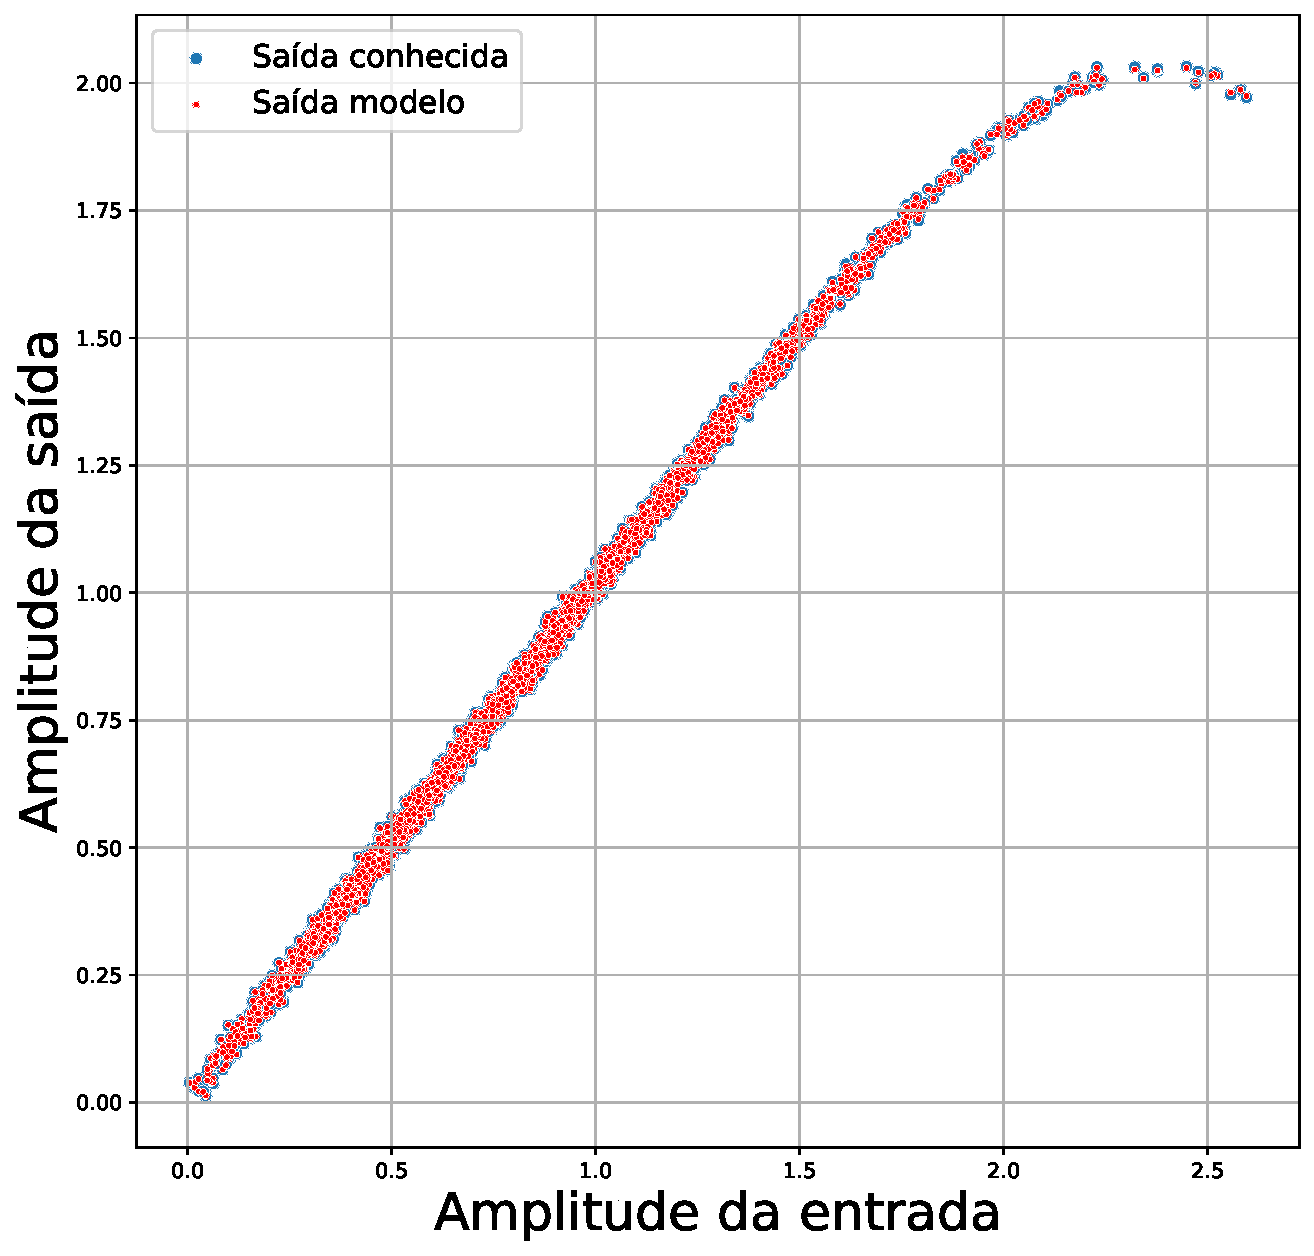
\includegraphics[width = 0.8\textwidth]{fig/extracao_pa.pdf}
}{O autor}{fig:extracao_pa}{}{Comparação gráfica entre as saídas conhecidas e as saídas do modelo para os dados de extração.}

A função de ativação foi a tangente hiperbólica, o total de entradas foi igual a 10, na camada de saída foi utilizada uma função de ativação linear, para a busca dos coeficientes foi utilizada a métrica MSE e o processo de busca usou o algoritmo Levenberg-Marquardt. Sendo a parte real e a parte imaginária treinadas separadamente.

O modelo foi capaz de ter um NMSE de -60.9 dB para os dados de treinamento e de -42.9 dB para os dados de validação. A \autoref{fig:extracao_pa} apresenta os valores da amplitude da saída em relação a entrada para os dados medidos e para os gerados pelo modelo para o conjunto de treinamento, enquanto a \autoref{fig:validacao_pa} mostra as mesmas informações para o conjunto de validação.

\imagem{Validação do PA}{
\label{fig:validacao_pa}
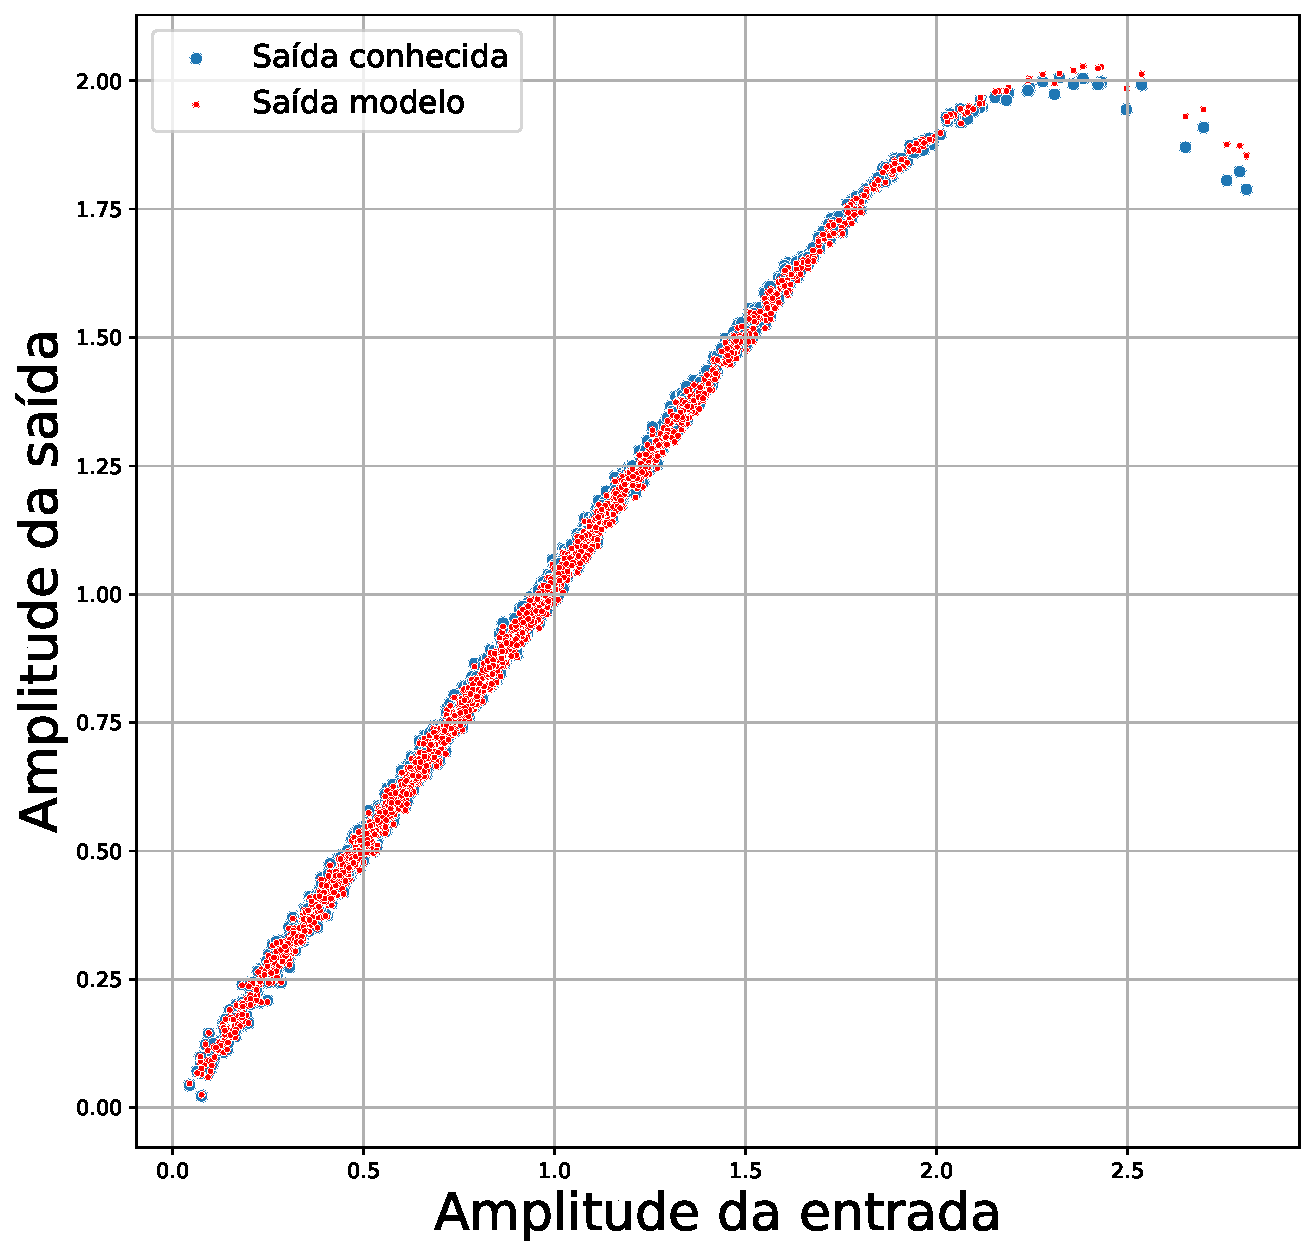
\includegraphics[width = 0.8\textwidth]{fig/validacao_pa.pdf}
}{O autor}{fig:validacao_pa}{}{Comparação gráfica entre as saídas conhecidas e as saídas do modelo para os dados de validação.}

\section{Uso do PI na análise do comportamento} \label{sec:estudoi-pi}

\subsection{Efeitos da continuidade da NN} \label{subsec:estudoi-pi-conti}
As redes neurais possuem a capacidade de generalizar o comportamento da função e estender esse comportamento para regiões não mapeadas, causando uma complicação adicional. Pois mesmo para entradas de menor amplitude, uma região descrente e não mapeada pode ser formada, como visto na \autoref{fig:continuidade_pa}. Um contorno a isso é penalizar a otimização na região não mapeada, multiplicando o erro encontrado por um coeficiente proporcional a amplitude de entrada proposto. Causar uma descontinuidade nessa região em testes preliminares se mostrou ineficiente e não foi adotado esse método.

\imagem{Continuidade do modelo}{
\label{fig:continuidade_pa}
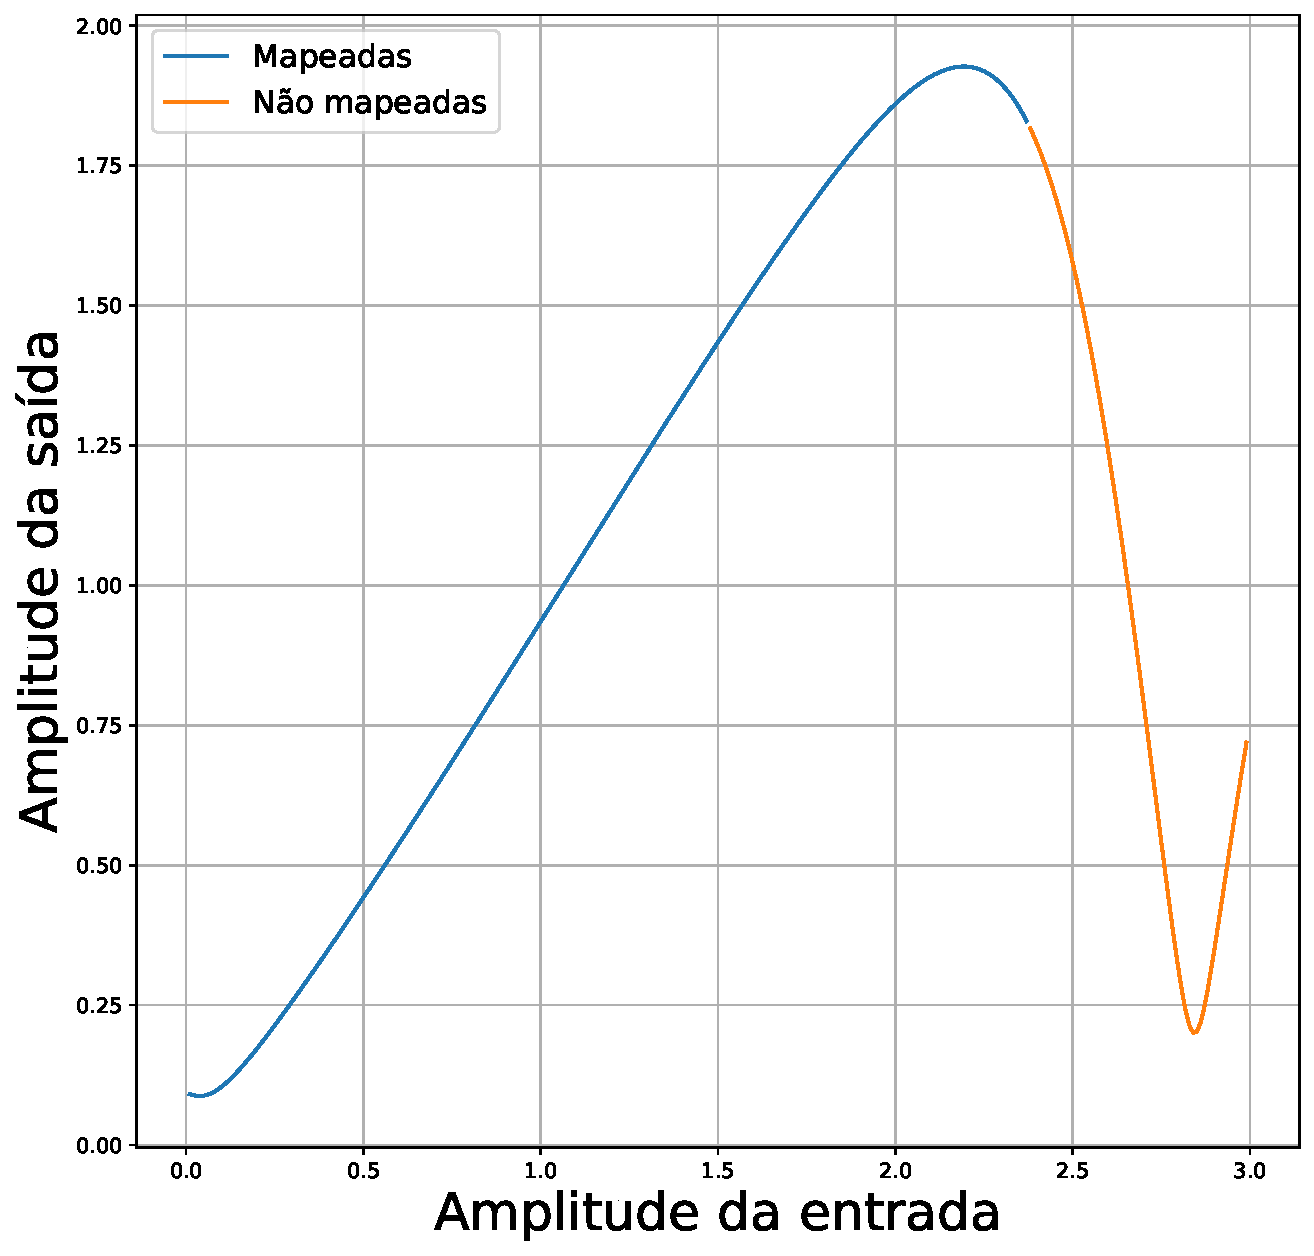
\includegraphics[width = 0.8\textwidth]{fig/continuidade_pa.pdf}
}{O autor}{fig:continuidade_pa}{}{Continuidade do modelo do PA com a memória fixada e variando-se a entrada entre 0 e 3, separando-se a região mapeada no treinamento e a região não mapeada no treinamento}

\subsection{Efeito dos valores iniciais na solução do PI e distribuição por amplitudes} \label{subsec:estudoi-pi-efeito}
Os 18 diferentes valores, presentes na \autoref{tab:valores}, foram definidos como chutes iniciais para o processo de solução do problema inverso. Sendo estes separados, junto aos resultados, em dois conjuntos: o primeiro conjunto com amplitude de 0,5 e segundo conjunto com amplitude de 2,5.

Nas \autoref{fig:erro_05} e \autoref{fig:erro_25} pode-se observar o comportamento destes dois principais conjuntos, no qual vemos a formação de três regiões. A região superior representa os valores que não convergiram, enquanto a inferior é dividida entre os que convergiram para o valor esperado e as que encontraram um valor de entrada não esperado. No gráfico está representado o erro entre o valor de saída e de entrada do modelo por meio do NMSE.

\imagem{Erros do problema inverso com chute inicial de 0,5}{
\label{fig:erro_05}
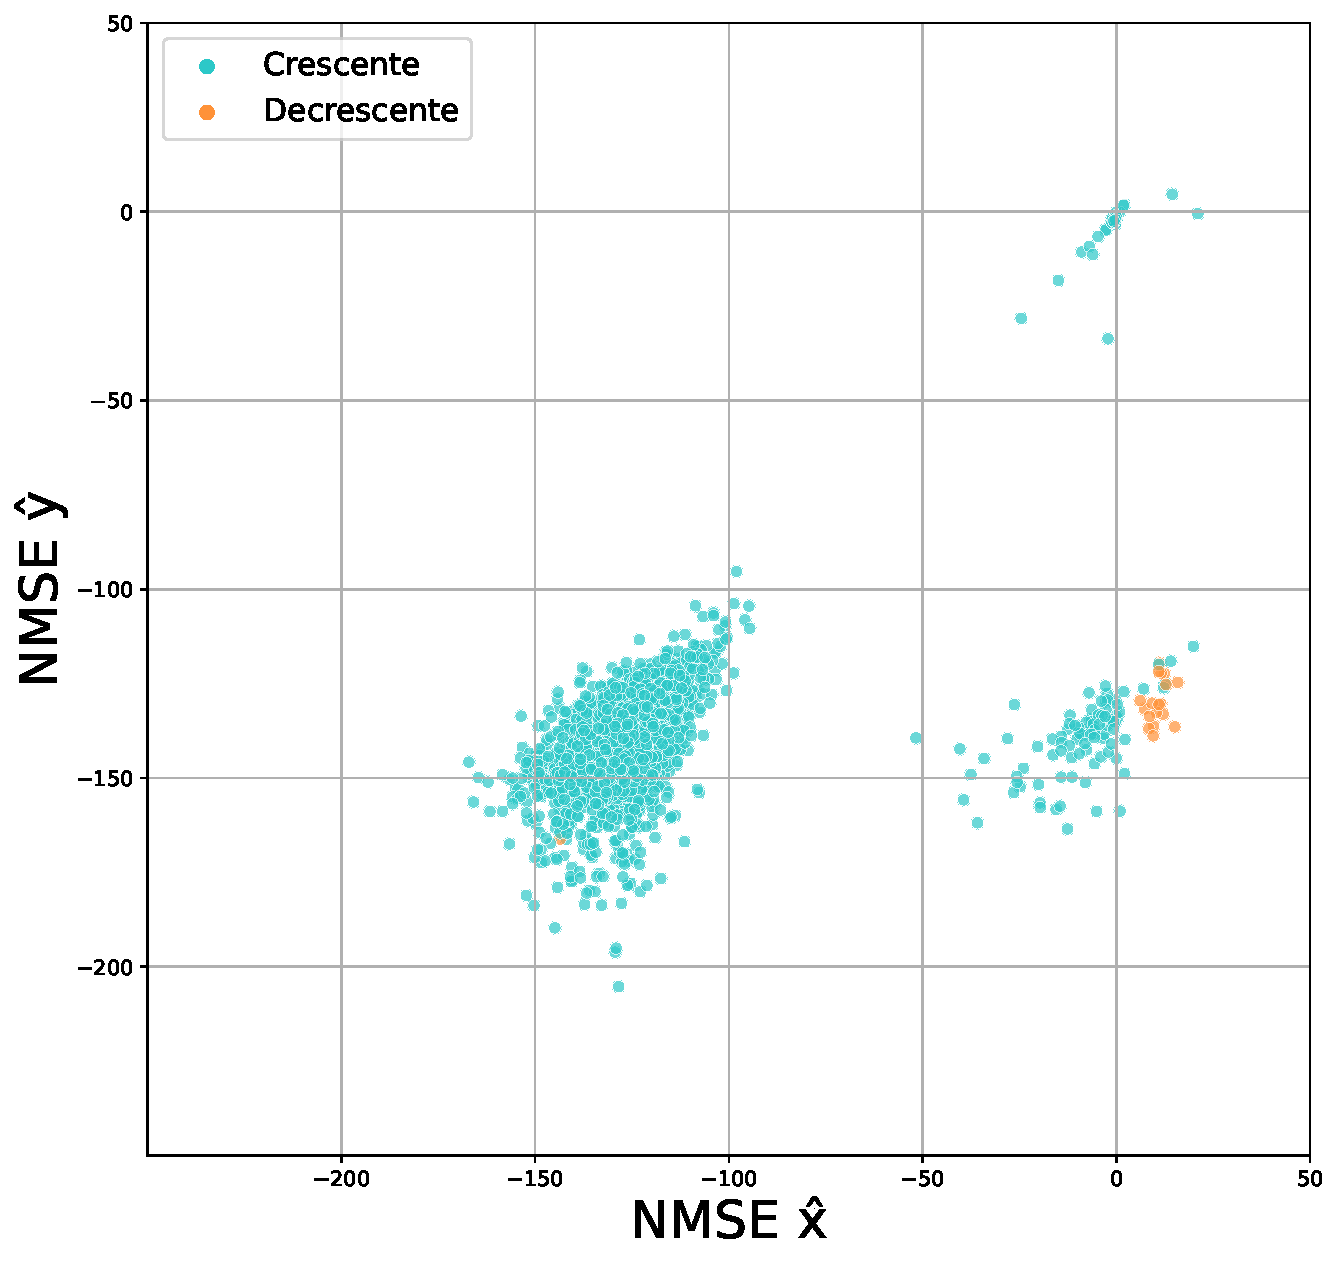
\includegraphics[width = 0.8\textwidth]{fig/erros_05.pdf}
}{O autor}{fig:erro_05}{}{Gráfico dos erros da entrada e da saída das soluções do problema inverso, com os resultados divididos nos três grupos analisados, para uma amplitude de 0,5.}

\imagem{Erros do problema inverso com chute inicial de 2,5}{
\label{fig:erro_25}
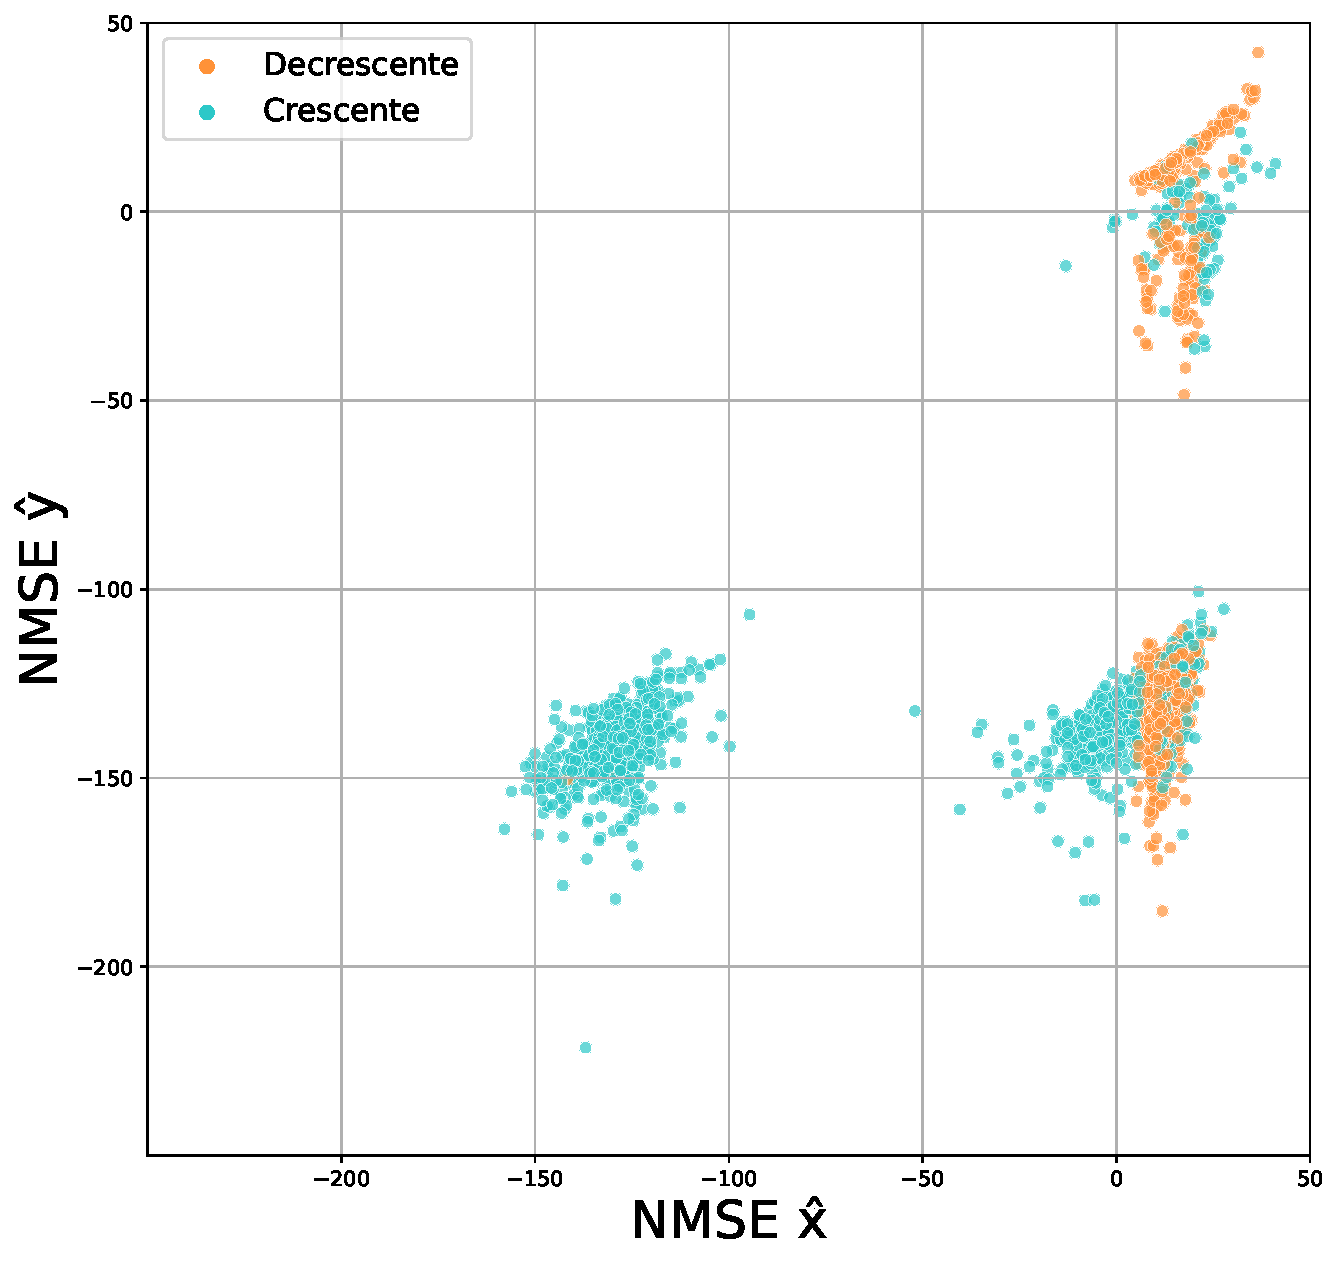
\includegraphics[width = 0.8\textwidth]{fig/erros_25.pdf}
}{O autor}{fig:erro_25}{}{Gráfico dos erros da entrada e da saída das soluções do problema inverso, com os resultados divididos nos três grupos analisados, para uma amplitude de 2,5.}

A distribuição por amplitudes e fases pode ser vista na \autoref{tab:valores_resultados05} para a amplitude de 0,5 e na \autoref{tab:valores_resultados25} para a amplitude de 2,5.
\tabela{Resultados para a amplitude 0,5}
{
\begin{tabular}{l|r|r|r}
    \hline
    \textbf{Valor inicial} & \textbf{Não convergiu} & \textbf{Falso} & \textbf{Correto} \\ \hline
    0,5$\angle$0 & 2,14\% & 3,14\% & 94,72\% \\ \hline
    0,5$\angle$2$\pi$/9 & 1,74\% & 3,51\% & 94,76\% \\ \hline
    0,5$\angle$4$\pi$/9 & 1,30\% & 3,71\% & 94,99\% \\ \hline
    0,5$\angle$6$\pi$/9 & 1,47\% & 3,04\% & 95,49\% \\ \hline
    0,5$\angle$8$\pi$/9 & 1,27\% & 3,67\% & 95,06\% \\ \hline
    0,5$\angle$10$\pi$/9 & 1,34\% & 3,27\% & 95,39\% \\ \hline
    0,5$\angle$12$\pi$/9 & 1,47\% & 4,18\% & 94,36\% \\ \hline
    0,5$\angle$14$\pi$/9 & 1,17\% & 3,97\% & 94,86\% \\ \hline
    0,5$\angle$16$\pi$/9 & 1,27\% & 4,04\% & 94,69\% \\ \hline
    \textbf{Média} & 1,46\% & 3,61\% & 94,92\% \\ \hline
    \end{tabular}
\label{tab:valores_resultados05}
}
{O autor}{tab:valores_resultados05}{}{Resultados para a amplitude 0,5}
\tabela{Resultados para a amplitude 2,5}
{
\begin{tabular}{r|l|l|l}
    \hline
        Valor inicial & Não convergiu & Falso & Correto \\ \hline
        2,5$\angle$0 & 16,70\% & 65,93\% & 17,37\% \\ \hline
        2,5$\angle$2$\pi$/9 & 15,36\% & 67,57\% & 17,07\% \\ \hline
        2,5$\angle$4$\pi$/9 & 15,76\% & 67,70\% & 16,53\% \\ \hline
        2,5$\angle$6$\pi$/9 & 17,33\% & 65,36\% & 17,30\% \\ \hline
        2,5$\angle$8$\pi$/9 & 16,83\% & 64,20\% & 18,97\% \\ \hline
        2,5$\angle$10$\pi$/9 & 17,74\% & 63,93\% & 18,34\% \\ \hline
        2,5$\angle$12$\pi$/9 & 16,13\% & 64,60\% & 19,27\% \\ \hline
        2,5$\angle$14$\pi$/9 & 14,96\% & 66,30\% & 18,74\% \\ \hline
        2,5$\angle$16$\pi$/9 & 15,90\% & 64,36\% & 19,74\% \\ \hline
        Média & 16,30\% & 65,55\% & 18,15\% \\ \hline
    \end{tabular}
\label{tab:valores_resultados25}
}
{O autor}{tab:valores_resultados25}{}{}

\subsection{Efeito das entradas para o problema inverso} \label{subsec:estudoi-pi-entradas}
Após se explorar o comportamento de todas as amostras para dezoito entradas diferentes, foi realizada uma análise para uma única amostra com amplitude de entrada igual a 2,58 e amplitude de saída igual a 1,99. Para essa amostra um total de 3600 entradas iniciais foram utilizadas, variando-se de forma constante o ângulo entre 0 e 6,18 e a amplitude entre 0 e 2,95.

Na \autoref{fig:calor_todos} vemos a amplitude encontrada para as diferentes resoluções do problema inverso, em razão da amplitude e do ângulo da entrada inicial.
\imagem{Amplitude do valor encontrado}{
\label{fig:calor_todos}
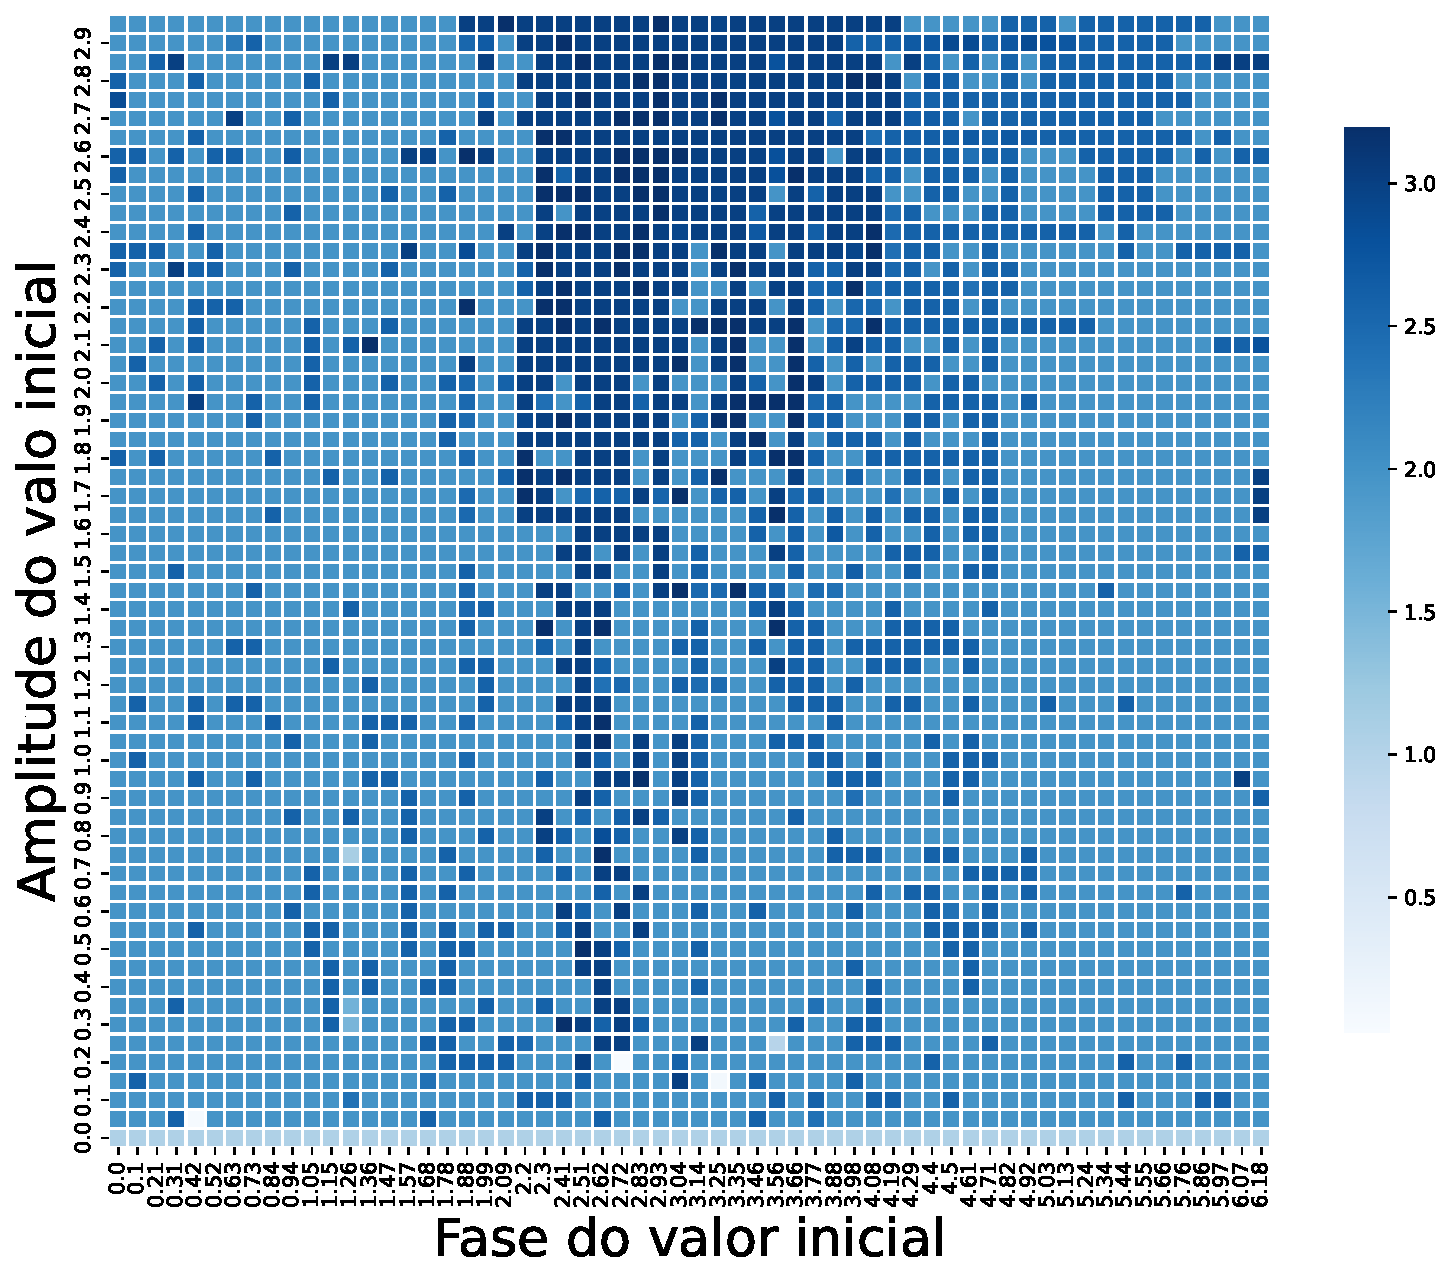
\includegraphics[width = 0.8\textwidth]{fig/calor_todos.pdf}
}{O autor}{fig:calor_todos}{}{}

No entanto, é necessário se excluir os pontos em que não ocorreu uma convergência, para isso analisamos o erro entre a saída do modelo e a saída ao ser aplicado o resultado do problema inverso, mostrado na \autoref{fig:calor_erro}.
\imagem{Erro do valor encontrado}{
\label{fig:calor_erro}
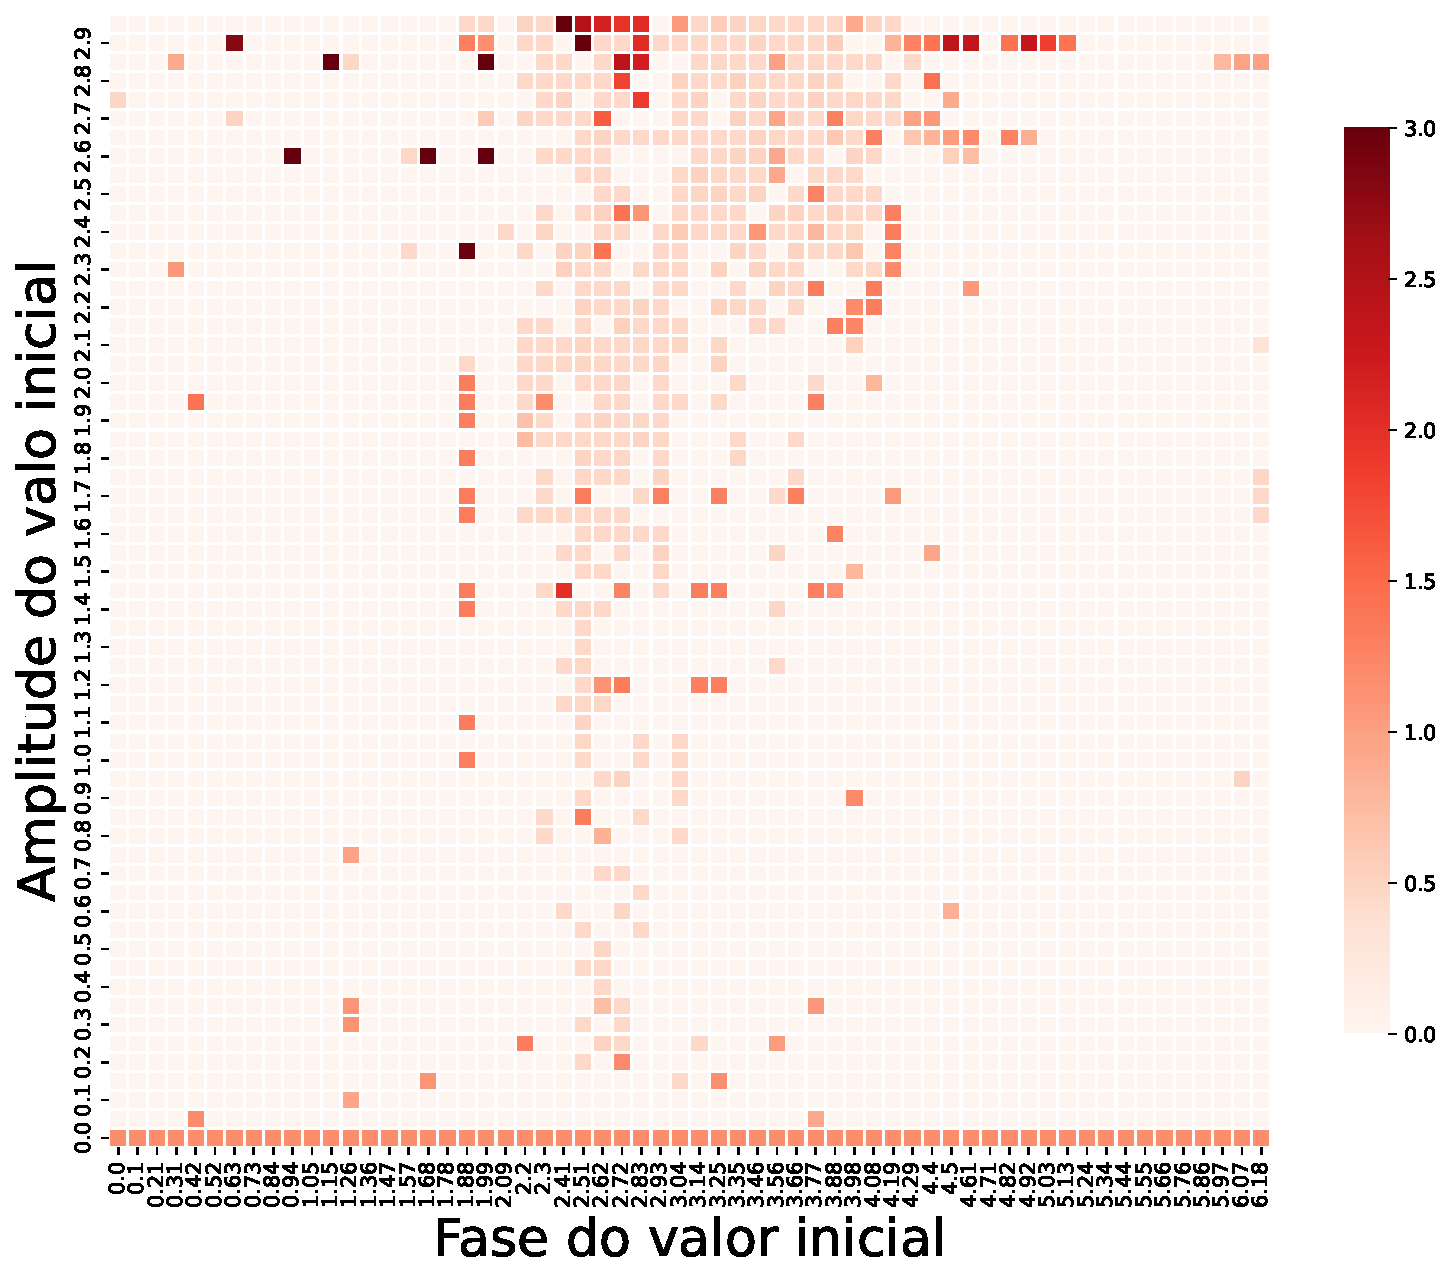
\includegraphics[width = 0.8\textwidth]{fig/calor_erro.pdf}
}{O autor}{fig:calor_erro}{}{}

Após o processo de exclusão destas amostras, que produzem um formato similar a um triangulo, obtemos como resultado a \autoref{fig:calor_converge}. Na qual podemos ver com clareza três resultados encontrados para a resolução do problema inverso, com o resultado correto sendo o prevalente para a maior parte dos pontos.
\imagemH{Amplitude do valor encontrado sem pontos divergentes}{
\label{fig:calor_converge}
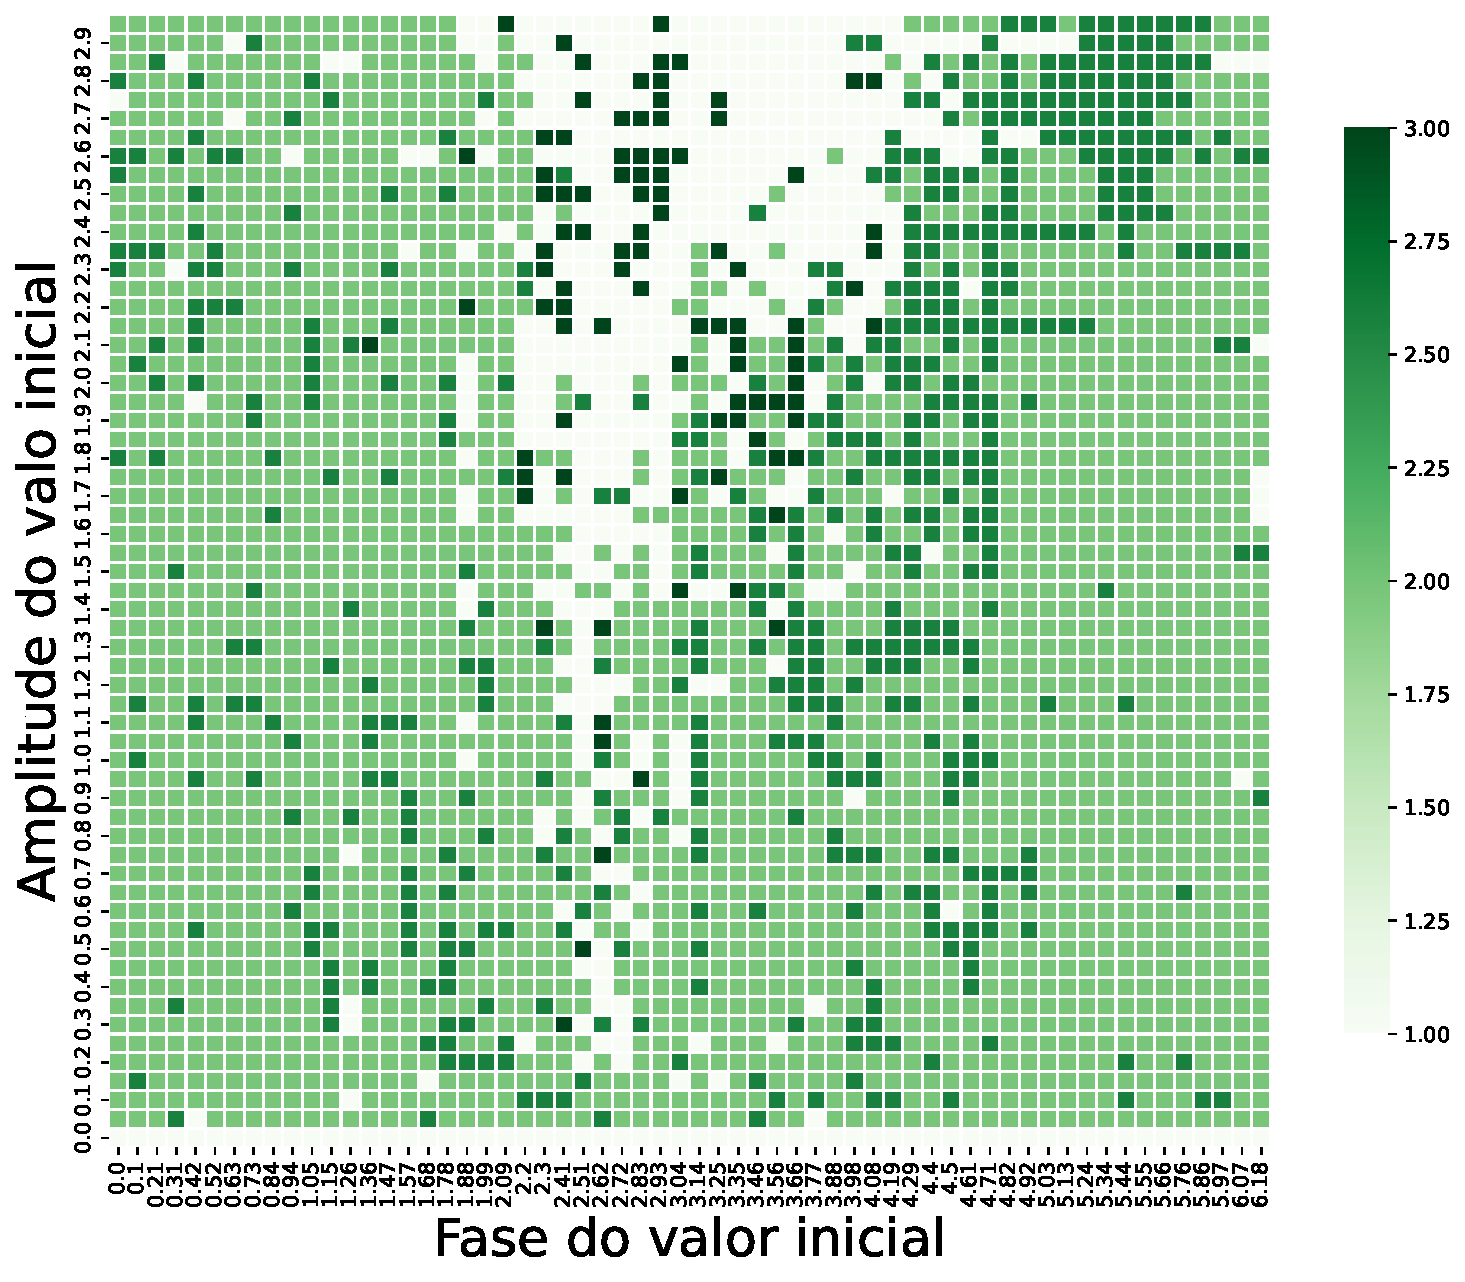
\includegraphics[width = 0.8\textwidth]{fig/calor_converge.pdf}
}{O autor}{fig:calor_converge}{}{}

\section{Treinamento da inversa} \label{sec:estudoi-inv}
Os resultados práticos no treinamento da inversa do PA através da mesma topologia, utilizando um valor de profundidade de memória M igual à 3 e uma quantidade de perceptrons na camada oculta HL igual à 7, deixam clara a maior dificuldade que o modelo inverso possui para generalizar os resultados na região não-linear e que mesmo o resultado do treinamento apresenta um desemprenho inferior ao do modelo direto. Isso pode ser observado graficamente nas \autoref{fig:extracao_inversa} e \autoref{fig:validacao_inversa}, respectivamente os dados de treinamento, com um NMSE de -51,33 dB, e de validação, com um NMSE de -26,48 dB.
\imagem{Extração da inversa}{
\label{fig:extracao_inversa}
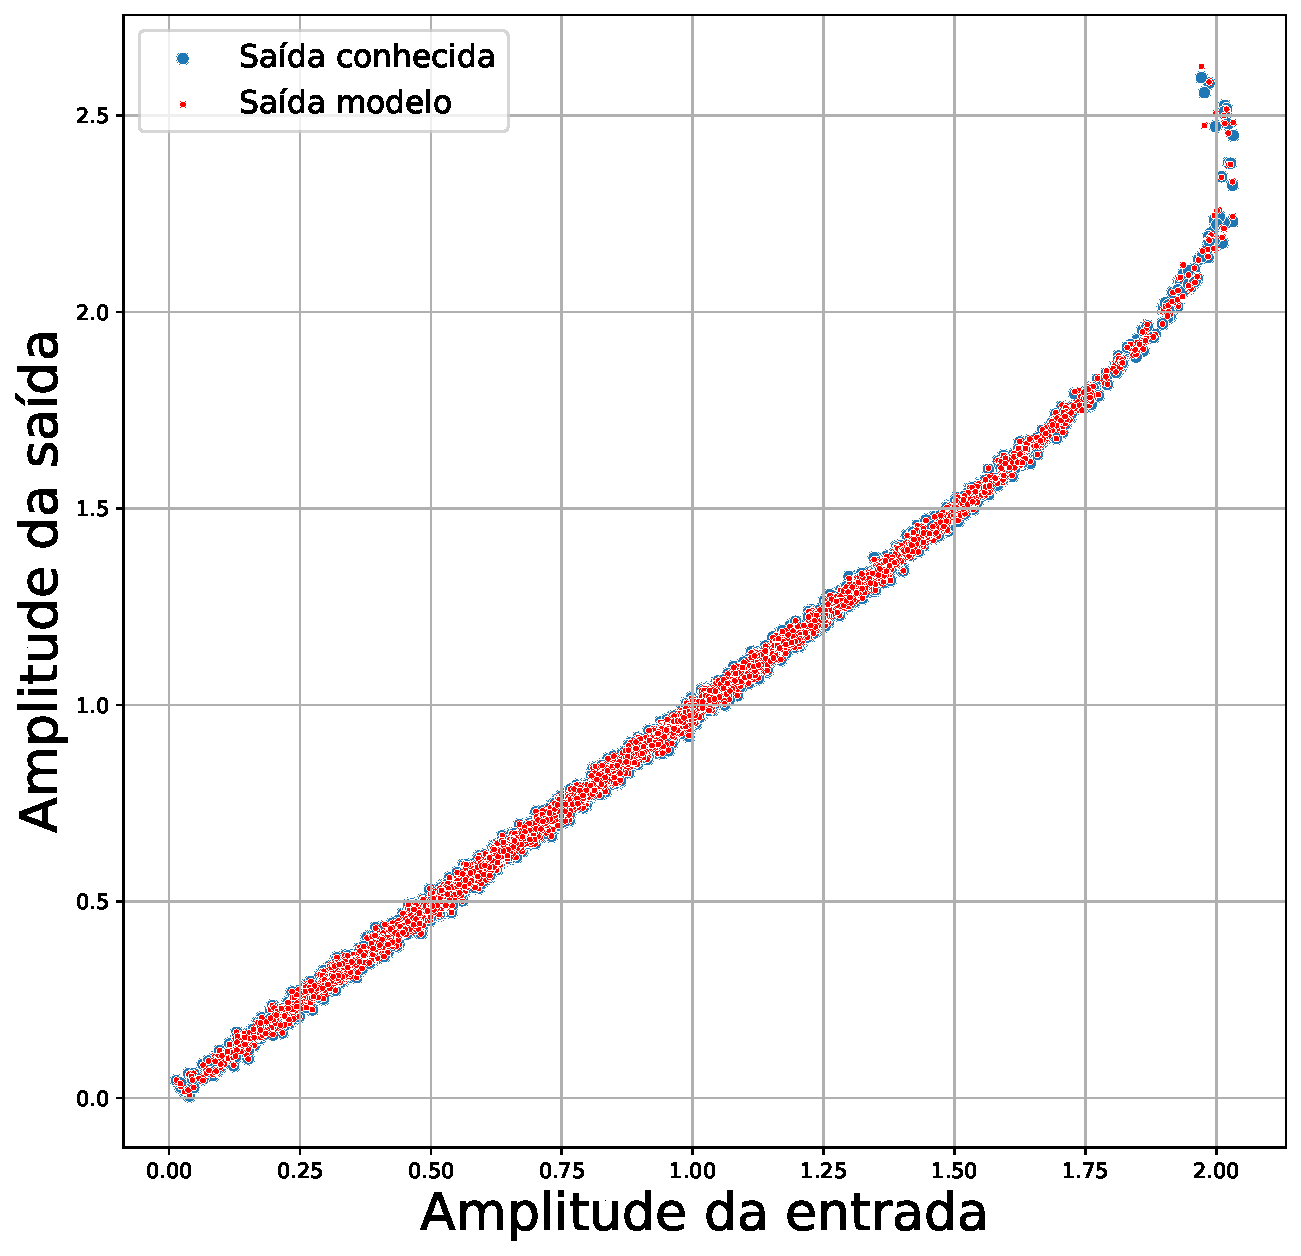
\includegraphics[width = 0.8\textwidth]{fig/extracao_inversa.pdf}
}{O autor}{fig:extracao_inversa}{}{Comparação gráfica entre as saídas conhecidas e as saídas do modelo da inversa do PA para os dados de extração.}
\imagem{Validação da inversa}{
\label{fig:validacao_inversa}
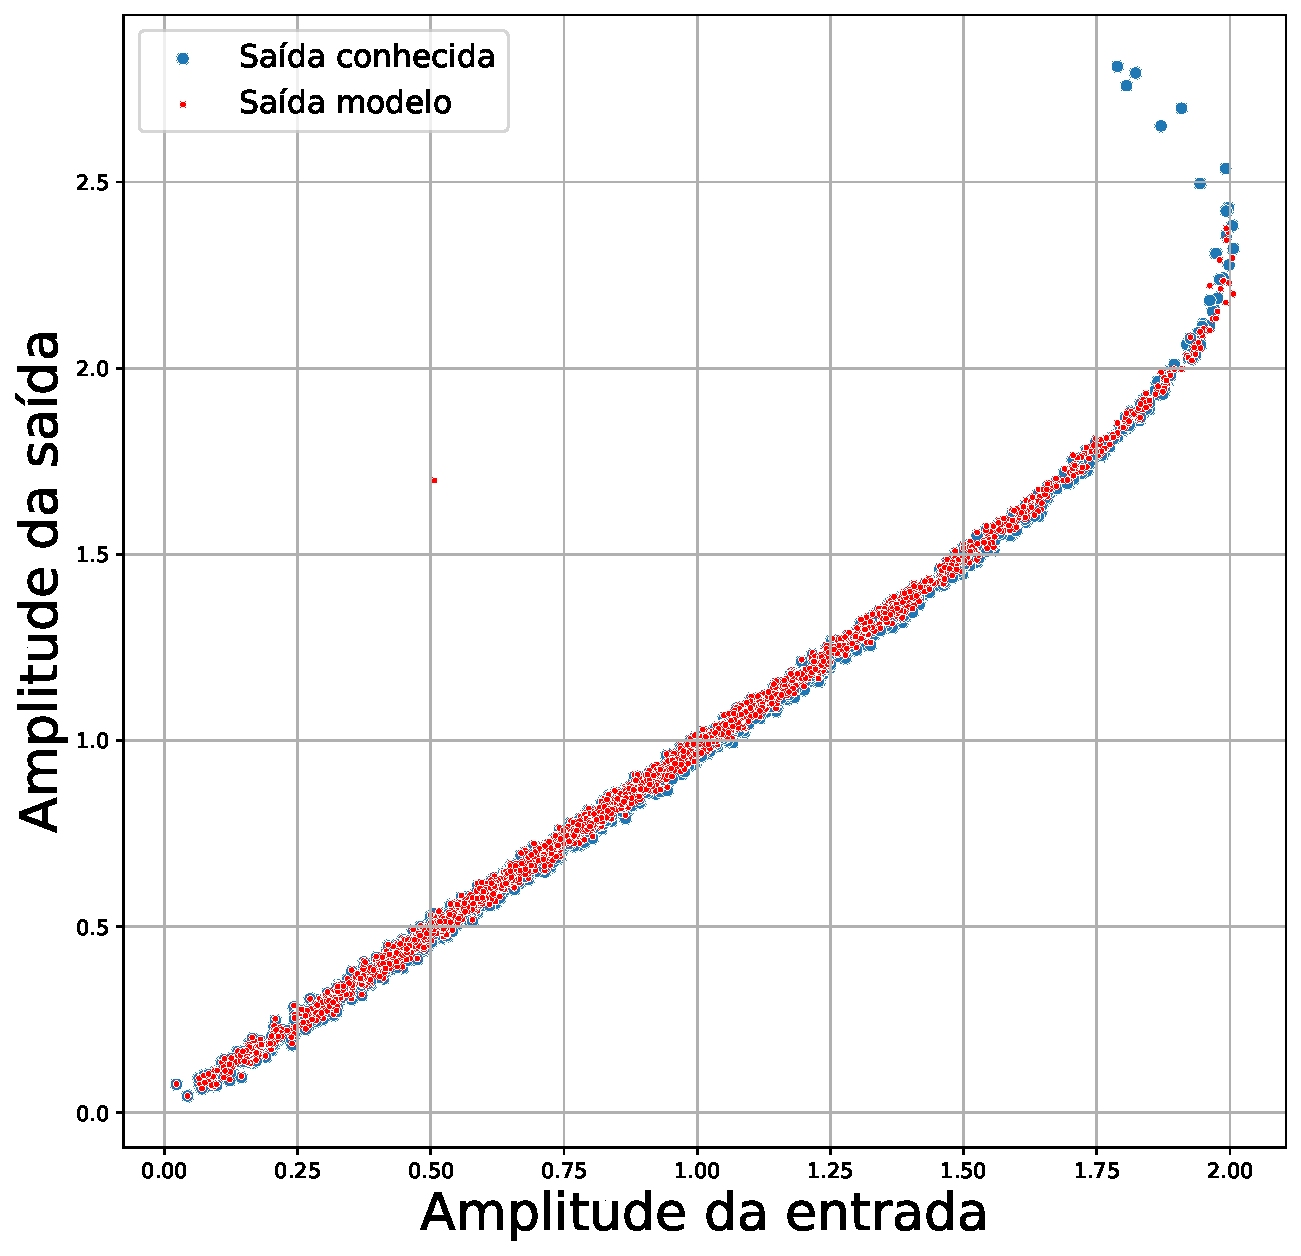
\includegraphics[width = 0.8\textwidth]{fig/validacao_inversa.pdf}
}{O autor}{fig:validacao_inversa}{}{Comparação gráfica entre as saídas conhecidas e as saídas do modelo da inversa do PA para os dados de validação.}

\chapter{Conclusão} \label{cha:conclusao}
O problema inverso se mostra através dos resultados presentes uma ferramenta promissora para a análise do comportamento de modelos computacionais de PAs e de suas inversas. Existe uma grande região para se aprofundar nestas análises, sendo esse estudo de caso somente uma pequena amostra das possibilidades, que já é capaz de auxiliar a delimitar as regiões mais estáveis em um modelo a partir da aplicação de diferentes amplitudes como parâmetro inicial no processo de resolução do problema inverso.
